\chapter{Design Science Research}
\label{chapter:DSR}

In this chapter, to answer the question ``Which projections can we create to help developers get appropriate feedback about rules?'' we undertook a design science research (DSR) approach.
In Section \ref{section:dsr_method}, we describe the method of this DSR.
Section \ref{section:dsr_results} examines the outcomes of our research.
Finally, in Section \ref{section:dsr_discussion}, we discuss the threats to the validity of our approach.

\section{Method - Drools in MPS}
\label{section:dsr_method}

Even though Drools is a relatively small DSL, we did not need to implement all the functionality to answer our questions.
For this reason, we first created a pilot study language to assess the possibilities of projectional solutions to our question.
We finally created a larger but incomplete version of Drools, in which we could create projections that would be recognisable to experienced Drools users.

\subsection{Really Simple Drools Language}
Our pilot study created a simple approximation of the Drools language to create our first projections. 
We called this language ``Really Simple Drools'' (RSD).
We describe this pilot study language here, as it contains many of the projections that we considered for our research question.

\paragraph{\texttt{File}} RSD, like Drools itself, has a \texttt{File} Concept as its root node.
The \texttt{File} Concept only contains \texttt{FactDeclaration} nodes and \texttt{Rule} nodes.

\paragraph{\texttt{FactDeclaration} and \texttt{FactProperty}} In Drools, a \texttt{FactDeclaration} Concept represents a Java Bean with its child properties, which can also have their child properties, ad infinitum.
In RSD, we limited properties to allow only boolean values.
We decided this because fact selection is a predicate and thus can only return a boolean.
By only allowing boolean values, we also simplify the operations allowed on a \texttt{FactProperty} node.

\paragraph{\texttt{Rule}} We only simulated the Left-hand side, or the ``when'' conditions, of a Drools Rule for the \texttt{Rule} Concept.
We believed this would provide us with compelling options for projections and did not want to overcomplicate this pilot project.

An RSD Rule consists of a collection of conditions.
Should all those conditions return ``true'', then the \texttt{Rule} node is selected.

\paragraph{\texttt{AbstractCondition}} A condition operates on one or more \texttt{FactSelectors} nodes.
There are four condition Concepts - \texttt{ExistsCondition}, \texttt{NotCondition}, \texttt{AndCondition}, and \texttt{OrCondition}.
The \texttt{ExistsCondition} and \texttt{NotCondition} Concepts are unary conditions and evaluate one \texttt{FactSelector} node.
The \texttt{AndCondition} and \texttt{OrCondition} Concepts evaluate two \texttt{FactSelector} nodes.

\paragraph{\texttt{FactSelector}} A \texttt{FactSelector} Concept consists of a reference to a \texttt{FactDeclaration} node and a collection of \texttt{AbstractPredicate} nodes.
If the fact exists and all the predicates evaluate to \texttt{true}, then the \texttt{FactSelector} evaluates to \texttt{true}.

\paragraph{\texttt{AbstractPredicate}} The predicate is an operation on a \texttt{FactProperty} node, to which the Concept has a reference.
Because \texttt{FactProperty} nodes represent a boolean value, the only predicate operations are ``And'', ``Or'', ``Is'', and ``Not''.

Figure \ref{fig:RSDDiagram} shows the Concept hierarch for this straightforward implementation.

\begin{figure}
    \centering
    \fbox{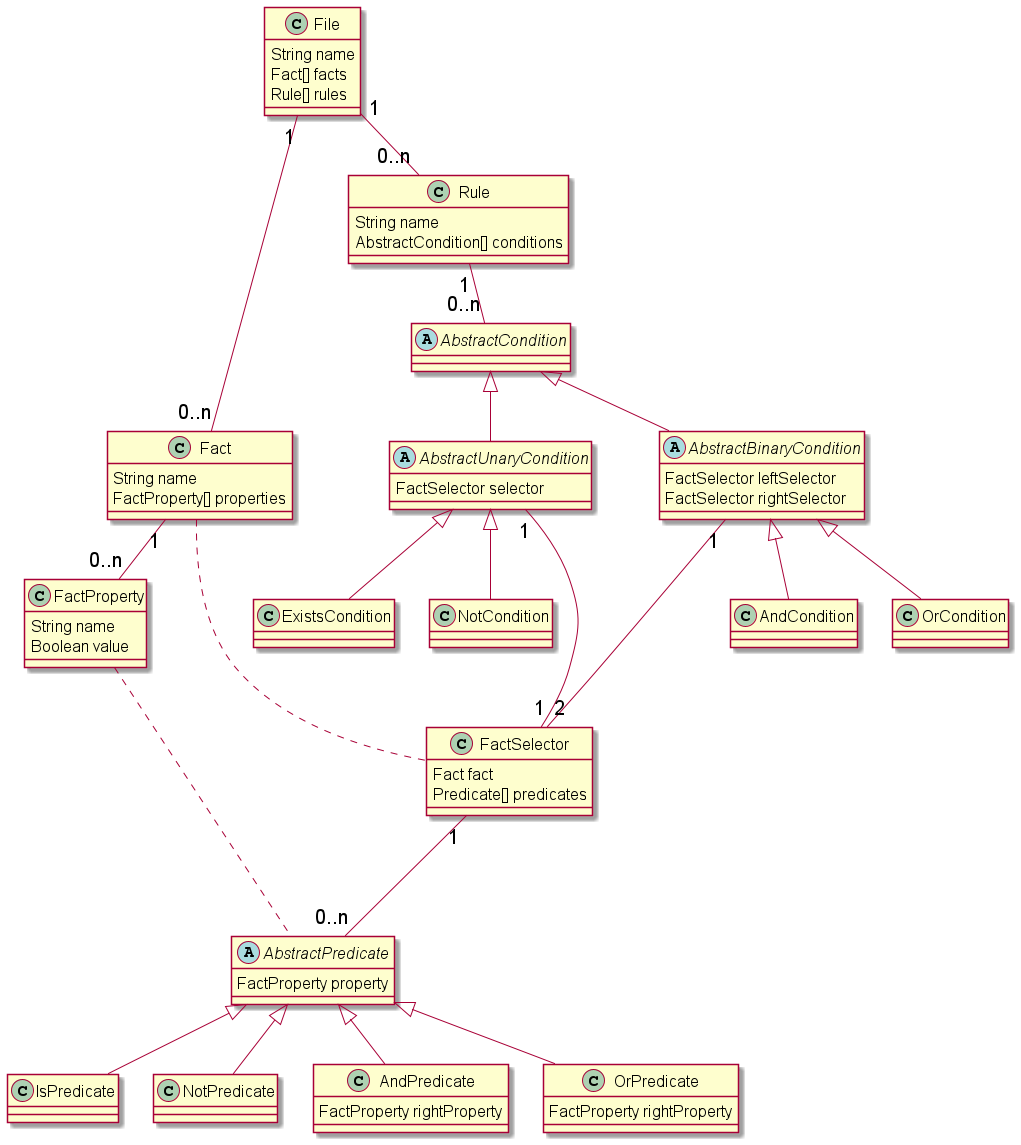
\includegraphics[width=0.95\textwidth]{Sections/images/ReallySimpleRuleLanguage4.png}}
    \caption{RSD concept hierarchy}
    \label{fig:RSDDiagram}
\end{figure}

We realised this design in MPS.
As the aim was to attempt different projections, we did not initially optimise for editing.
The Structure is as shown in figure \ref{fig:RSDStructure}.
We have here translated our Conceptual design of the RSD into MPS Concepts.
There is an almost one to one relationship with our concept hierarchy diagram.
The one difference is that the references in the concept hierarchy diagram, represented by the dashed red lines, are represented in our MPS Structure by SmartRef Concepts \texttt{FactDeclarationSmartRef} and \texttt{FactPropertySmartRef}.

\begin{figure}[h]
    \centering
    \fbox{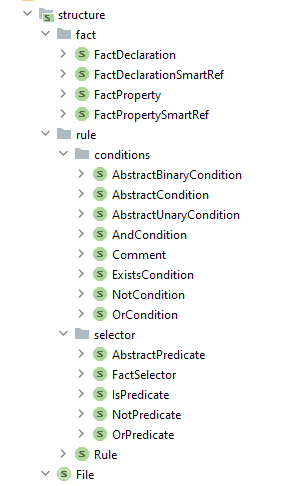
\includegraphics[width=0.40\textwidth]{Sections/images/RSRStructrure.png}}
    \caption{RSD Language Structure}
    \label{fig:RSDStructure}
\end{figure}

We show the definitions of the editors in figure \ref{fig:RSDEditors} on the following page. 
The first editor describes the \texttt{File} Concept. 
It shows that the first line will have the text ``rule file name: '' followed by the file's name.
Following an empty line, there is a vertical listing of the \texttt{FactDeclaration} nodes stored in the ``facts'' child of the \texttt{File} node.
Thereafter is another empty line followed by a vertical listing of the \text{Rule} nodes stored in the ``rules'' child.

The next editor shown is the editor of the \texttt{FactDeclaration} Concept.
Each \texttt{FactDeclaration} node will be shown on a single line starting with the word ``fact'' followed by its name.
Then, between parentheses, a horizontal, comma-separated list of its child \texttt{FactProperty} nodes.

The subsequent editor describes the \texttt{Rule} Concept. 
The layout it describes is similar to that of a Drools rule, with the first line being ``rule'' followed by the \texttt{Rule} node name in inverted commas.
There is a hardcoded indented ``when'', followed by a further indented vertical list of the condition children, which are \texttt{AbstractCondition} nodes.
At appropriate indentation levels, the conditions are followed by three hardcoded lines of ``then'', a comment as a place holder for the right-hand side of a standard Drools rule, and ``end''.

Next, we show one of the \texttt{AbstractCondition} Concepts, in this case, the \texttt{AndCondition} Concept.
This Concept editor displays the two \texttt{FactSelector} child nodes separated by ``and'' and surrounded by parentheses.

The editor for the \texttt{FactSelector} Concept displays the fact child, which is a \texttt{FactDeclarationSmartRef} node, for which we do not show its editor here, but in this case, shows the name of the \texttt{FactSelector} node that it is referencing.
The name is followed by a horizontal, comma-separated list of the \texttt{AbstractPredicate} nodes stored in the predicate's children, encased in parentheses.

The final editor we show is an example of an \texttt{AbstractPredicate} Concept, specifically an \texttt{OrPredicate} Concept, which shows the two properties separated by a ``||'' symbol.
The properties are \texttt{FactPropertySmartRef} nodes, and they will just display the name of the \texttt{FactProperty} node to which they point.

\begin{figure}
    \centering
    \fbox{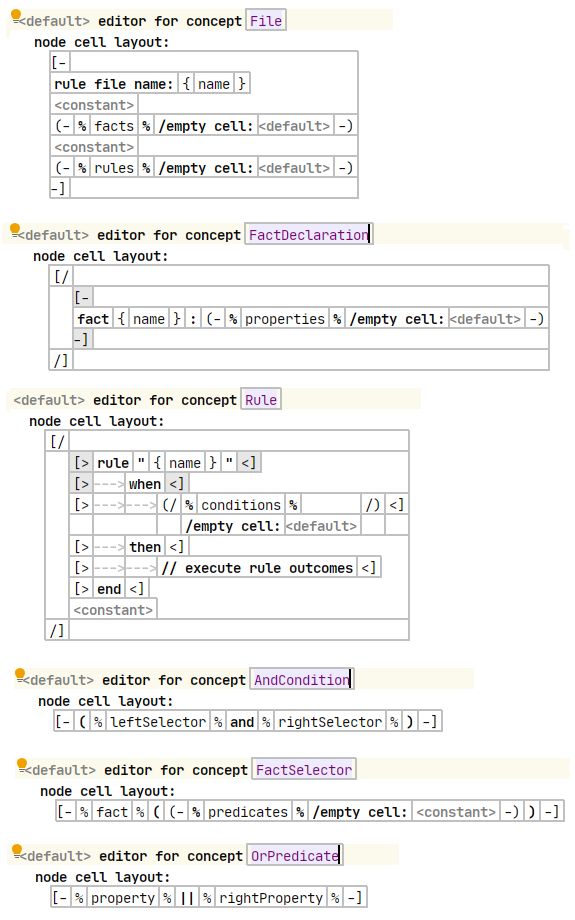
\includegraphics[width=0.66\textwidth]{Sections/images/RSREditors_P2.png}}
    \caption{Editors}
    \label{fig:RSDEditors}
\end{figure}

\newpage

We show the result of the editors in figure \ref{fig:RSDProgram}, which shows an example of our default Drools-like text projection. 
This projection is of the root AST of a \texttt{File} node called ``DossierSleutelbos''.
It has 4 \texttt{FactDeclaration} child nodes and 3 \texttt{Rule} child nodes.
The \texttt{FactDeclaration} nodes called ``Dossier'', ``Episode'', and ``Milestone'' each have two child \texttt{FactProperty} nodes, whilst ``DroolsContext'' has none.

The \texttt{Rule} node ``0'' has 2 \texttt{ExistsCondition} nodes containing \texttt{FactSelector} node children with \texttt{FactDeclarationSmartRef} nodes referencing the \texttt{FactDeclaration} nodes ``Dossier'' and ``DroolsContext''.

The \texttt{Rule} node ``[WVGGZ/CM] start CM Procedure'' points to the ``Dossier'' \texttt{FactDeclaration} node, as well as having two predicates.
The first predicate is an \texttt{IsPredicate} node with a \texttt{FactPropertySmartRef} node pointing to the ``isWvGGZ'' \texttt{FactProperty} node.
The other predicate is a \texttt{NotPredicate} node pointing to the ``hasRunningEpisode'' \texttt{FactProperty} node.

The final \texttt{Rule} node has a complex nesting of \texttt{AbstractCondition} nodes.
The first is an \texttt{OrCondition} node containing an \texttt{ExistsCondition} node on its left-hand side and an \texttt{AndCondition} node on the right.
The right-hand side node contains an \texttt{ExistsCondition} node on both the left and right sides. 

\begin{figure}[h]
    \centering
    \fbox{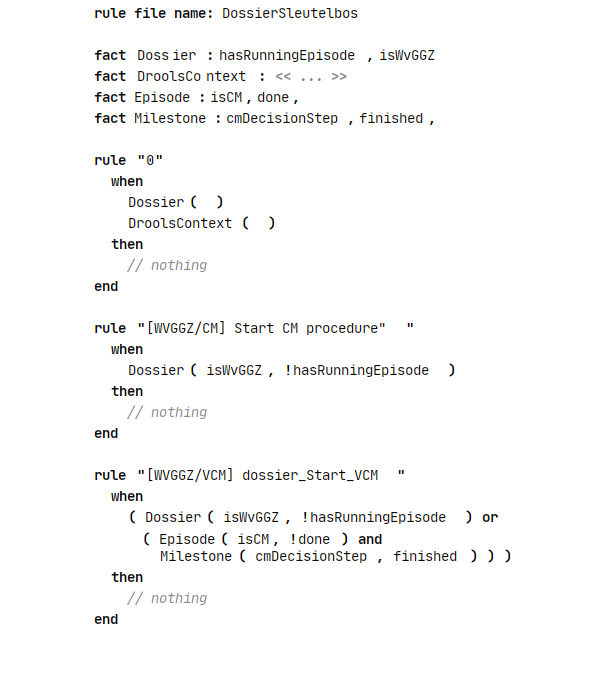
\includegraphics[width=0.66\textwidth]{Sections/images/RSRProgram_P.png}}
    \caption{RSD program}
    \label{fig:RSDProgram}
\end{figure}

\newpage

Part of our research question is using projections for reasoning about large files.
To answer this, we needed to simulate a large file.
To do this, we had to enter many \texttt{Rule} nodes.
As this becomes tedious, we added some editing aids, including substitute menus, to speed up the entry of Conditions, as shown in figure \ref{fig:RSDSubstituteMenu}.

\begin{figure}[h]
    \centering
    \fbox{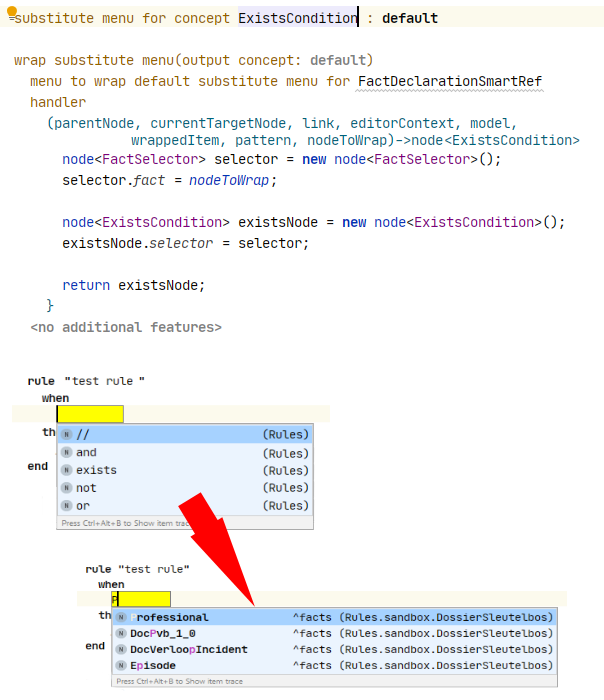
\includegraphics[width=0.66\textwidth]{Sections/images/RSRSubstituteMenu_P.png}}
    \caption{RSD substitute menu}
    \label{fig:RSDSubstituteMenu}
\end{figure}

This image shows that we originally had to select an \texttt{ExistsCondition} Concept and select the \texttt{FactDeclaration} node for the Condition.
After adding the substitute menu, we could immediately select the \texttt{FactDeclaration} node we wanted, and it would automatically wrap it with an \texttt{ExistsCondition} node.

We show the code to do this in the section ``wrap substitute menu''.
What it does is when it encounters the possibility to input an \texttt{ExistsCondition} node in a menu, it replaces it with the default menu for the \texttt{FactDeclarationSmartRef} Concept.
MPS handles SmartRefs in menus by showing all the possible reference items available.
When the user picks the reference item, this code will create a new \texttt{ExistsCondition} node with a new \texttt{FactSelector} node containing the chosen \texttt{FactDeclarationSmartRef} node to insert at that point in the AST.
This substitute menu saves several keystrokes, as otherwise, we manually first had to insert an \texttt{ExistsCondition} node followed by a \texttt{FactSelector} node before filling the \texttt{FactDeclaration} child.

Finally, we added a Constraint to scope the \texttt{FactProperty} references in \texttt{Predicate} Concept to the \texttt{FactDeclaration} reference chosen in the \texttt{FactSelector} node.
This scope Constraint made it much easier to select \texttt{FactProperty} nodes in a \texttt{Predicate} node, as indicated in figure \ref{fig:RSDConstraint}.

\begin{figure}
    \centering
    \fbox{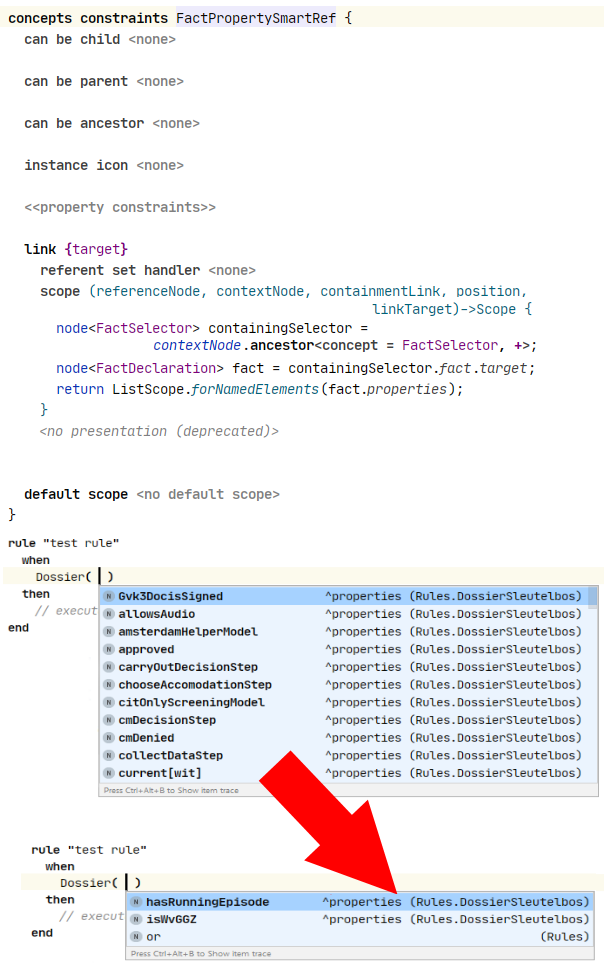
\includegraphics[width=0.66\textwidth]{Sections/images/RSRConstraint_P.png}}
    \caption{RSD scoping constraint}
    \label{fig:RSDConstraint}
\end{figure}

The figure shows that before adding the scoping constraint, it showed a list with dozens of potential \texttt{FactProperty} nodes representing all the \texttt{FactProperty} nodes in the model.
After adding the constraint, it only shows the two \texttt{FactProperty} references associated with the \texttt{FactDeclaration} referenced in the \texttt{FactSelector}.
We achieve this scoping in the code in the scope method.
The code first finds the relevant \texttt{FactDeclaration} node from the \texttt{FactSelector} node we are at in the AST.
From this, it returns a list of properties as a \texttt{Scope}.

Thus, we have described the entire implementation of the Really Simple Drools Language.

After implementing the language, we wrote a program with many rules.
This program on which we will experiment with the different projections.

We discuss the alternative projections in the results section \ref{section:dsr_results}.

\newpage
\subsection{Drools-Lite Language}
\label{section:DroolsLite}

The RSD was useful as an initial language. 
However, it suffered from two significant issues.
Firstly, its limitations as a language were so substantial that it could not handle many necessary scenarios.
Secondly, our projections would be validated by developers with Drools experience, and RSD would be too alien to them.
For this reason, we needed to create a projectional language that was much closer to the Drools language.

\begin{figure}
    \centering
    \fbox{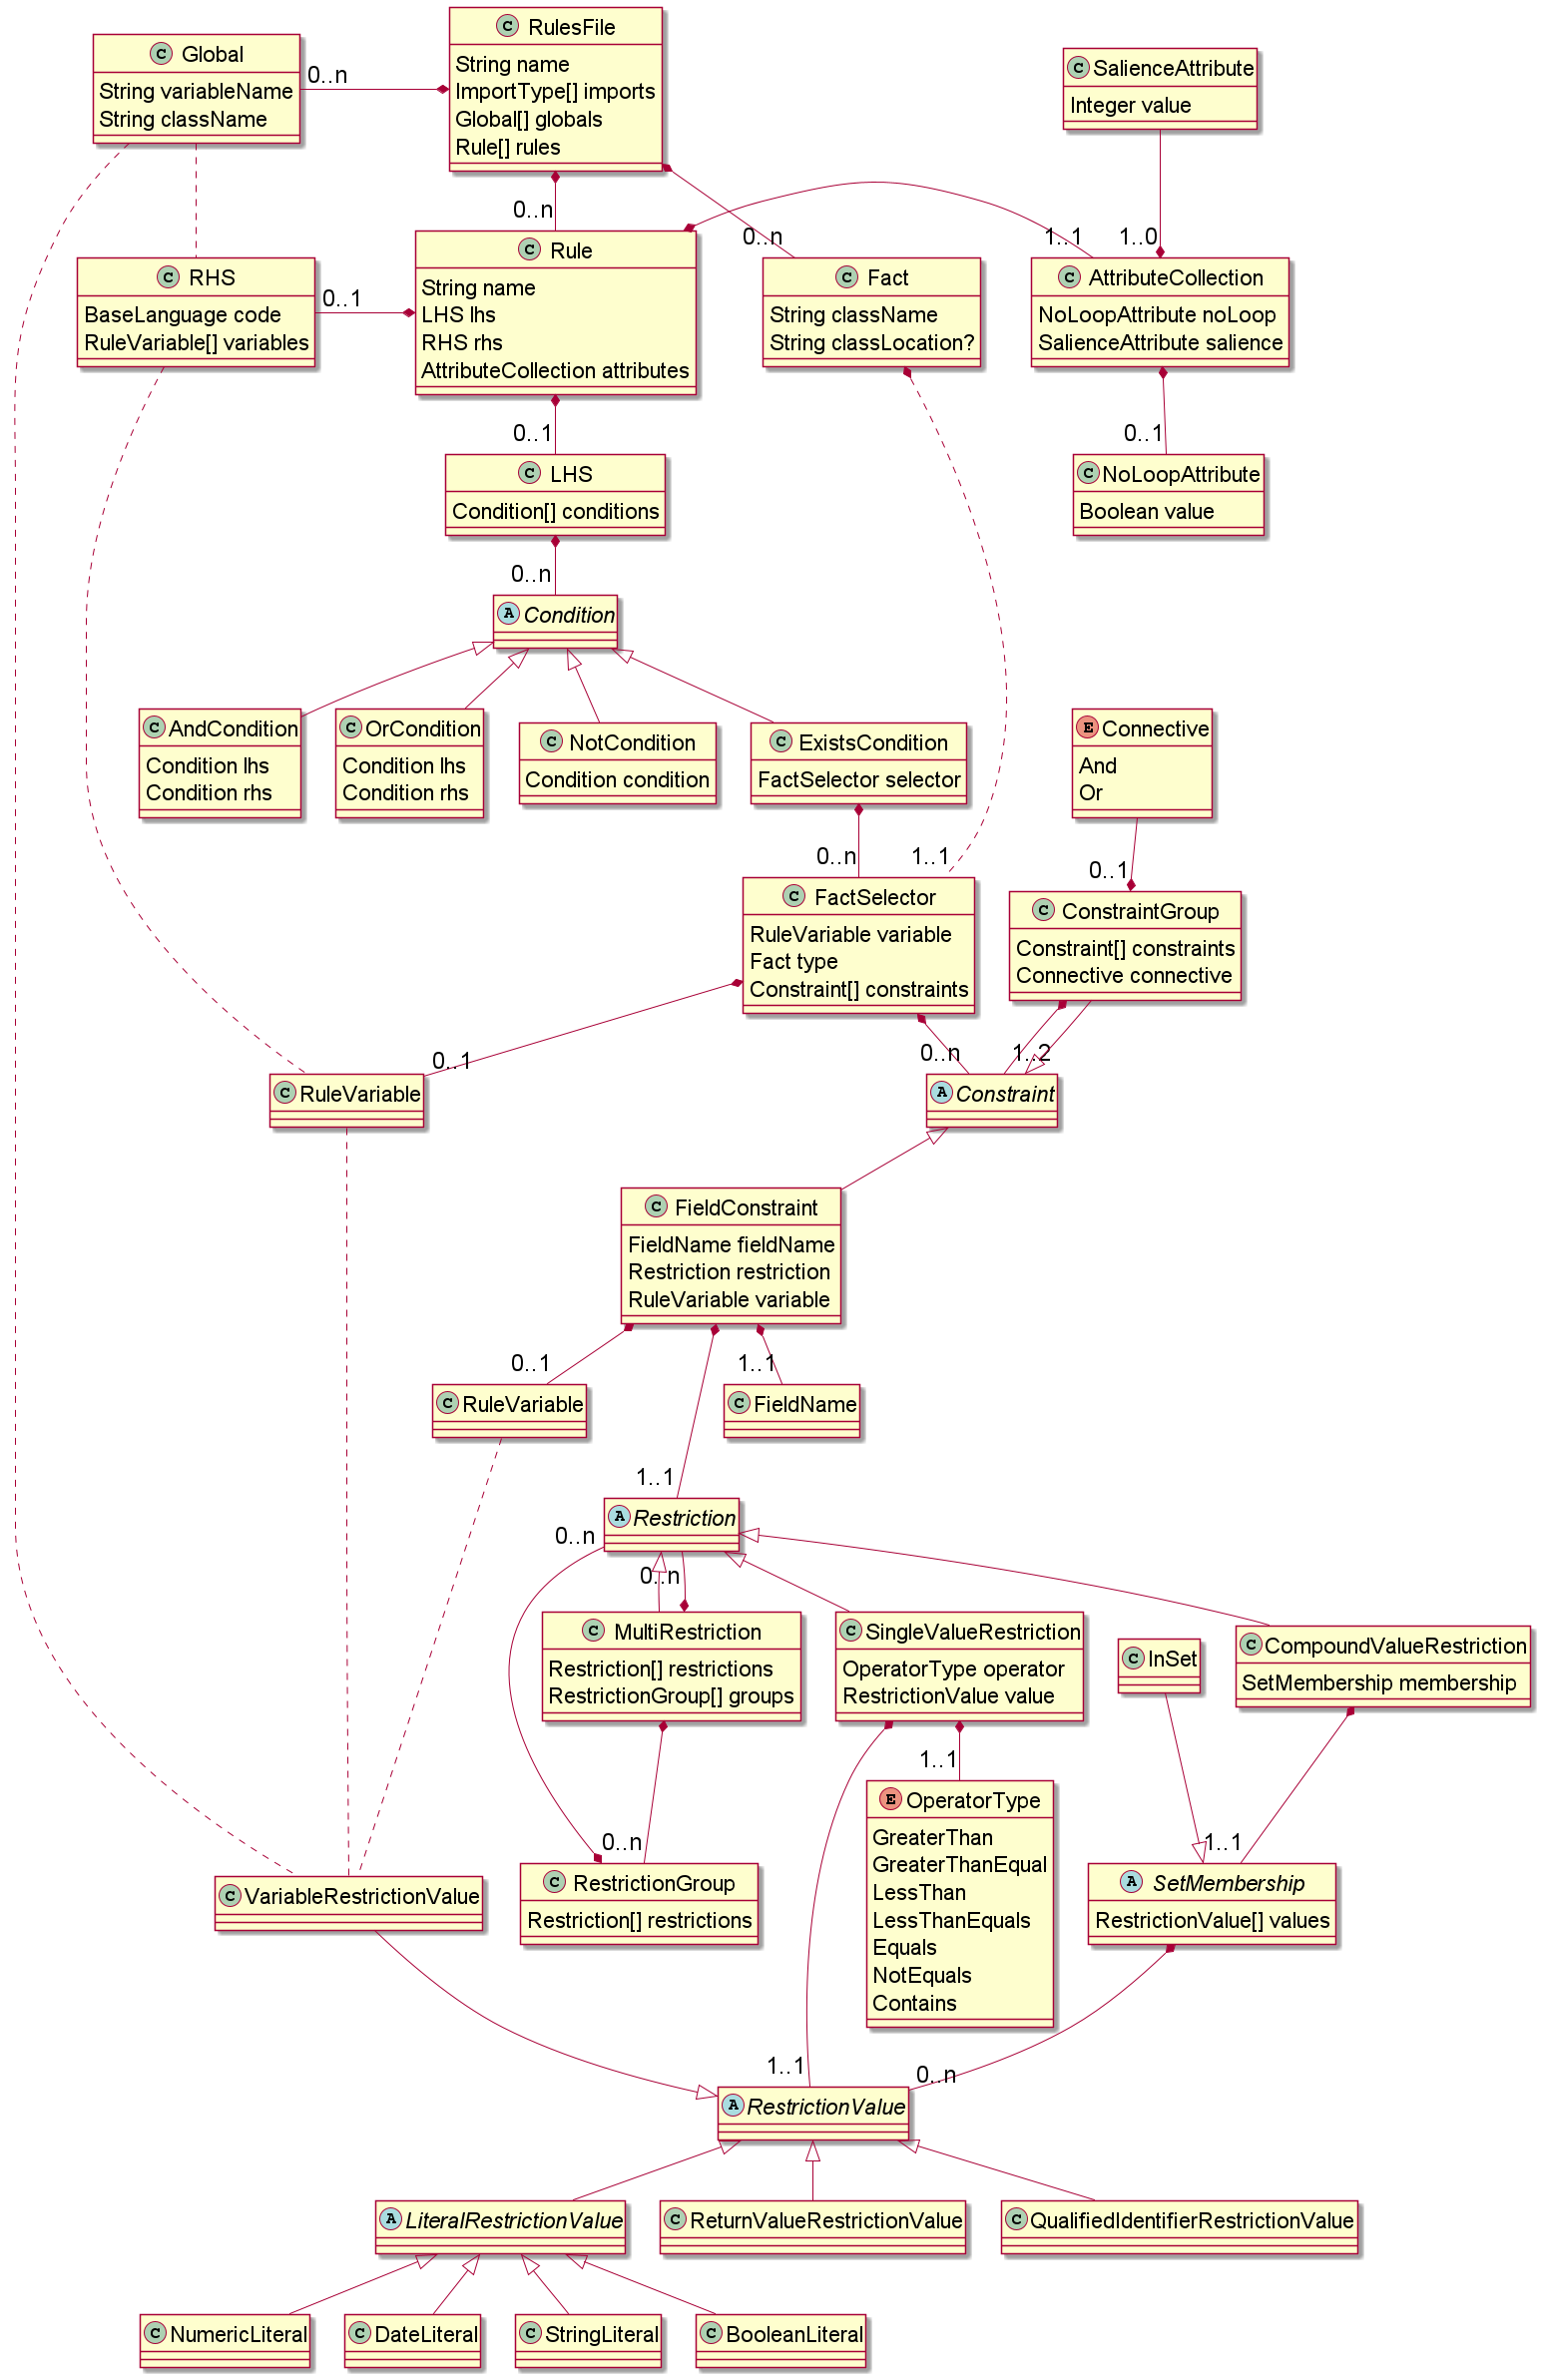
\includegraphics[width=0.90\textwidth]{Sections/images/DroolsLiteStructure.png}}
    \caption{Drools-Lite structure}
    \label{fig:DroolsLiteDiagram}
\end{figure}
 
Our following Language, Drools-Lite, contains many more of the features of Drools.
Our method of selecting the features involved implementing the examples delivered with Drools (including the corrupt politician example shown in section \ref{section:WhatIsDrools}).
We would implement just enough features to complete the examples.
Whenever we had any queries about designing Concepts, we referred to our analysis of the Drools Language, shown in appendix \ref{appendix:DroolsConceptHierarchy}.
We show the preliminary design we achieved using this method in figure \ref{fig:DroolsLiteDiagram} on page \pageref{fig:DroolsLiteDiagram}.
Later, there were some places we diverged a little from our design.
We merged and decoupled our Concepts when we thought it would simplify the code.

\paragraph{\texttt{RuleFile}} The \texttt{RuleFile} Concept contains \texttt{FactDeclaration} nodes, \texttt{Global} nodes and \texttt{Rule} nodes.
It also contains semantically unimportant empty lines.

\paragraph{FactDeclaration} A \texttt{FactDeclaration} Concept has a \texttt{type} property.
We implement the \texttt{type} property using a \texttt{ClassifierType} node from the MPS BaseLanguage.
This implementation allows a \texttt{RuleFile} node to refer to BaseLanguage classes implemented in the same solution or from Java JAR files.

We created a smart reference Concept for this to take advantage of built-in MPS UI functionality.
A smart reference is a node with a single reference of 1:1 cardinality.
The editor builders know how to select which nodes are in scope to display to the developer if one uses this object rather than directly referencing the node it refers to.

\paragraph{FactProperty} In RSD, we had \texttt{FactProperty} nodes as children of \texttt{FactDeclaration} nodes.
Now that our \texttt{FactDeclaration} nodes refer to actual classes (\texttt{ClassifierType}), our \texttt{FactProperty} Concept should reflect this.
To do this, the Concept itself only references an \texttt{InstanceMethodDeclaration}, the MPS BaseLanguage's definition of a method signature.
We scoped the Concept to only show properties associated with a selected \texttt{FactDeclaration}.

Drools interacts with Java objects as if they are Java Beans.
To simulate this, we limited the scope of the properties to just getters, i.e., methods that start with ``get'' or ``is'', and used a Behavior to make sure they are displayed without the ``get'' or ``is'' prefix.
We also made a smart reference for this Concept.

Another option for achieving this is to have wrapped the \texttt{ClassifierType} Concept and referenced its related \texttt{InstanceMethodDeclarations}.
We would have then had to limit the functionality of these items from the BaseLanguage.
Whilst this allows the functionality we wished for, we feel our construction offers decoupling and that, we think, correctly reflects the structure of the language.
Perhaps if we were to redo this, we would have taken the other approach.

\paragraph{\texttt{Global}} Our \texttt{Global} Concepts are very simple.
They have a ``name'' property and a BaseLanguage \texttt{Type} child node.
We added a smart reference so that \texttt{Rule} nodes can easily use them.
The reference extended the \texttt{Expression} Concept from the BaseLanguage.
This extension is so that we could use it in the Java code of the Right-hand side.

\paragraph{\texttt{Rule}} Our \texttt{Rule} Concept has three children: an \texttt{AttributeCollection} node, a Right-hand side node and a list of \texttt{AbstractConditions} that make up the Left-hand side.
We created a component to describe the \texttt{Rule} editor for reuse, as we imagined that we would wrap this in other projections.

\paragraph{\texttt{RuleVariables}} The \texttt{FactDeclaration} node referenced by a \texttt{FactSelector} node and the \texttt{FactProperty} referenced by a \texttt{FieldConstraint} node can be bound to \texttt{RuleVariable} nodes.
\texttt{RuleVariable} nodes are scoped to a \texttt{Rule} node.
A \texttt{RuleVariable} Concept has only a \texttt{name} property and a \texttt{Type} child node.
We also create a smart reference for it so that it can be used elsewhere within the \texttt{Rule}.
Like the \texttt{Global} Concept, it extends BaseLanguage's \texttt{Expression} to be available in the Java code of the Right-hand side.

\paragraph{Right-hand side} The right-hand side of the \texttt{Rule}, for the most part, is Java code.
To implement this, we made the right-hand side of the \texttt{Rule} Concept a single \texttt{StatementList} node.
A \texttt{StatementList} Concept is a list of \texttt{Statements} nodes, both from the BaseLanguage.
We chose these because they keep track of, amongst other things, scope of variables among the statements.

There are some non-Java, Drools specific items that are available to the right-hand side.
Items that had to be useable within the right-hand side were \texttt{Global} references, \texttt{RuleVariable} references and Drools specific functions.
These all extend \texttt{Expression} Concept from the BaseLanguage.
This extension allows seamless integration with the Java code.

The Drools specific methods that are required are represented by the \texttt{Insert}, \texttt{InsertLogical}, \texttt{Modify}, \texttt{Delete} and \texttt{Halt} Concepts.

\begin{figure}[h]
    \centering
    \fbox{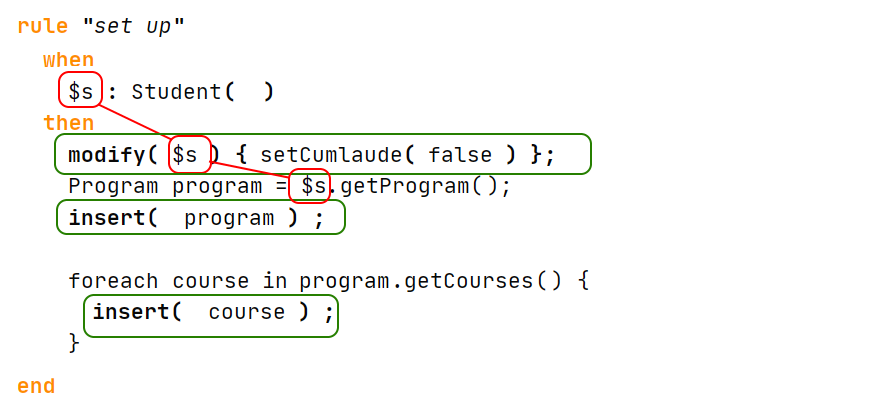
\includegraphics[width=0.70\textwidth]{Sections/images/RHS.png}}
    \caption{RHS}
    \label{fig:RHS}
\end{figure}

Figure \ref{fig:RHS} shows some of the features discussed for the right-hand side, as shown in our default projection.
The right-hand side is the text shown between the ``then'' keyword and the ``end'' keyword.
The figure shows examples of plain Java code, such as assigning to the variable ``program'' and the ``foreach'' loop.
We can also see that Drools-Lite \texttt{RuleVariable} node ``\$s'' is in the Java statements.
We have also highlighted the Drools specific methods placed in the code, in this case \texttt{\textbf{modify}} and \texttt{\textbf{insert}}   

\begin{figure}[h]
    \centering
    \fbox{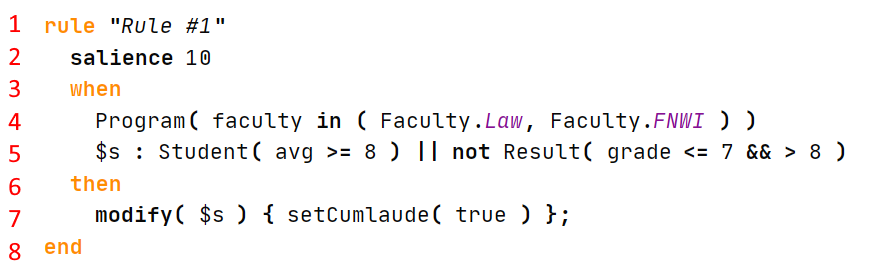
\includegraphics[width=0.85\textwidth]{Sections/images/Rule.png}}
    \caption{Rule}
    \label{fig:Rule}
\end{figure}

\paragraph{\texttt{AttributeCollection}} The \texttt{AttributeCollection} Concept is a container to hold all the attributes that apply to a \texttt{Rule} node.
Initially, we have only implemented the \texttt{NoLoopAttribute} and \texttt{SalienceAttribute} Concepts.
A developer activates these attributes using two intentions we added to the \texttt{Rule} Concept.
On line 2 in figure \ref{fig:Rule}, we can see an example of a \texttt{SalienceAttribute} node added to a \texttt{Rule} on line 2.
\footnote{In figure \ref{fig:Rule}, we added line numbers to this figure to make it easier to talk about.
The keywords ``rule'' on line 1, ``when'' on line 3, ``then'' on line 6, and ``end'' on line 8 have no meaning in the abstract syntax.
We added them to give the developer the same look and feel as a standard Drools file.}

\paragraph{Left-hand side} This is a collection of \texttt{AbstractCondition} nodes.
There are four types of \texttt{AbstractCondition} Concepts.
\texttt{AndCondition}, \texttt{OrCondition}, \texttt{NotCondition} and \texttt{ExistsCondition} Concept.
\texttt{AndCondition}, \texttt{OrCondition}, and \texttt{NotCondition} have one or two children who are also \texttt{AbstractCondition} nodes.
The \texttt{ExistsCondition} Concept contains a \texttt{FactSelector} node.

We added dynamic braces to only show braces around a Condition if it is a child of another Condition.
These braces add visual clarity without adding unnecessary clutter.
We also added some intentions to make it easy to switch between \texttt{ExistsCondition} and \texttt{NotCondition} nodes.

On line 4 in figure \ref{fig:Rule}, the whole line represents an \texttt{ExistsCondition} node.
Line 5 shows an \texttt{OrCondition} node containing an \texttt{ExistsCondition} node and a \texttt{NotCondition} node.
The default editor, through an intention, can make the \texttt{ExistsCondition} visibly explicit with an ``exists'' keyword.
However, the standard practice with Drools developers is to make this implicit, so this is how we show it here.

\paragraph{\texttt{FactSelector}} This always has a reference to a \texttt{FactDeclaration} node.
These are references to the \texttt{FactDeclaration} nodes named ``Program'' in line 4 of figure \ref{fig:Rule} and ``Student'' and ``Result'' from line 5.

Optionally, the \texttt{FactSelector} node can be bound to a variable.
In figure \ref{fig:Rule}, line 5, the \texttt{FactSelector} node referencing the \texttt{FactDeclaration} named ``Student'' is bound to the \texttt{RuleVariable} node named ``\$s''.

The \texttt{FactSelector} Concept also contains a list of constraints on \texttt{FactProperty} references, all of which must return true for a \texttt{FactSelector} node to return true.

\paragraph{Constraints} We have three types of \texttt{AbstractConstraint} Concepts.
\texttt{AndConstraint} and \texttt{OrConstraint} Concepts contain other child constraints.
The \texttt{FieldConstraints} Concept places restrictions on \texttt{FactProperty} references.

\paragraph{FieldConstraints} A \texttt{FieldConstraint} Concept refers to a \texttt{FactProperty} node and can be bound to a variable.
It also has a restriction applied to that \texttt{FactProperty} node.
Using a substitute menu, we wrapped the \texttt{FactPropertySmartRef} Concept.
This substitution automatically creates a \texttt{FieldConstraint} node from the \texttt{FactProperty} node selection by the developer.

There are several types of restrictions and several types of values that they can restrict.

\paragraph{\texttt{RestrictionValues}} The \texttt{AbstractRestrictionValue} Concepts that a \texttt{FactProperty} node can be compared with are as follows:
\begin{itemize}    
    \setlength\itemsep{0em}
    \item \texttt{LiteralRestrictions}: These are \texttt{Integer}, \texttt{Float}, \texttt{String}, \texttt{DateTime} and \texttt{Boolean}.
    \item \texttt{VariableRestrictions}: These can be \texttt{Global} references, \texttt{RuleVariable} references referring to \texttt{FactDeclaration} references from the \texttt{FactSelector} node, or  a\texttt{RuleVariable} node from other \texttt{FieldConstraint} nodes.
    \item \texttt{ReturnValue}: This compares to anything expressed as an \texttt{Expression}, which includes referring to constants or values behind qualified identifiers.
\end{itemize}

In figure \ref{fig:Rule}, on line 4, we have the return values ``Faculty.Law'' and ``Faculty.FNWI''.
On line 5, the literal values ``7'' and ``8''.

\paragraph{Restrictions} A \texttt{SingleValueRestriction} Concept compares a \texttt{FactProperty} node against a value.
A \texttt{MultiRestriction} Concept compares a \texttt{FactProperty} node against multiple values, not necessarily using the same comparison for each value.
A \texttt{SetMembership} restriction Concept checks if a \texttt{FactProperty} node is a member or not a member of a group.

In figure \ref{fig:Rule} on line 4 a \texttt{SetMembership} restriction node is shown with the ``in ( Faculty.Law, Faculty.FNWI )'' text.
Line 5 in the first \texttt{FactSelector} node there is the \texttt{SingleValue} restriction node represented by ``avg >= 8''.
The second \texttt{FactSelector} node shows a \texttt{MultiRestriction} node using ``grade <= 7 \&\& > 8''.

Thus, we have described the pertinent implementation details of the Drools-Lite language.

\subsection{Wireframes}

There are some potential projections we have conceived for which there is not sufficient time to implement.
We want Drools experts to assess these and thus would like them to appear as realistic as possible to the assessors.

Our solution to this conundrum is to develop these presentations in a wireframing tool.
The wireframe tool we chose was Axure\cite{Axure_ProductPage}.
We chose this because we had previous experience with the product.
Also, it is available to students for free.

We settled on two possible projectional programming aids: Truth table and circuit diagram.
We will discuss these in more detail in the results section.


\section{Results}
\label{section:dsr_results}

\subsection{Really Simple Drools}

The Really Simple Drools Language (RSD) acted as a training ground for our new projections.

\subsubsection{Context-Aware Colour Scheme}
After the default text projection, the first projection we made was giving the text a colour scheme.
This form or augmentation in IDEs is probably the most basic that we see.
Available in structured editors since the 1980s\cite{cowlishaw1987lexx}, syntax highlighting displays text in various colours and fonts according to the meaning of the terms.
Syntax highlighting is helpful for the comprehension of code, as least for small code bases\cite{sarkar2015impact}.

Developers at our host organisation use Eclipse or IntelliJ Community Editions to edit code, neither of which has syntax highlighting for Drools. Thus, the addition of this feature would immediately benefit them.
However, IntelliJ IDEA, the paid version, already provides this feature for Drools.
We extended the colour scheme to indicate whether the selection is looking for a positive or negative match to offer another visual augmentation that we considered valuable.
Figure \ref{fig:colorscheme} shows this projection.

\begin{figure}[h]
    \centering
    \fbox{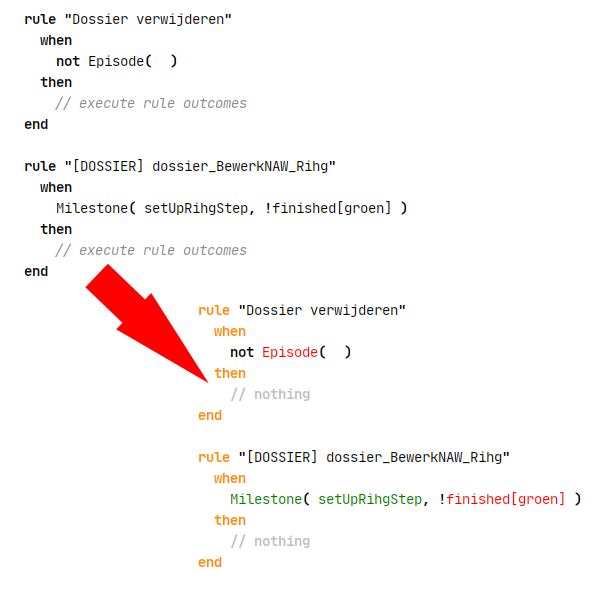
\includegraphics[width=0.66\textwidth]{Sections/images/coloredTextProjection_P.png}}
    \caption{Context aware colour scheme}
    \label{fig:colorscheme}
\end{figure}

\texttt{FactDeclaration} references contained by \texttt{NotCondition} nodes and \texttt{FactProperty} references that are part of a \texttt{NotPredicate} node appear highlighted in Red.
\texttt{ExistCondition} and \texttt{IsPredicate} nodes have their content coloured green.
We did not test whether this improved understanding.

\subsubsection{Summary Projection}

Our next projection allows developers to have a quick overview of the \texttt{Rule} nodes and the complexity of those nodes.
Figure \ref{fig:summaryProjection} shows that the developers can get an overview of both the number of \texttt{Rule} nodes and the number of \texttt{FactDeclaration} references in each of the \texttt{Rule} nodes.

\begin{figure}
    \centering
    \fbox{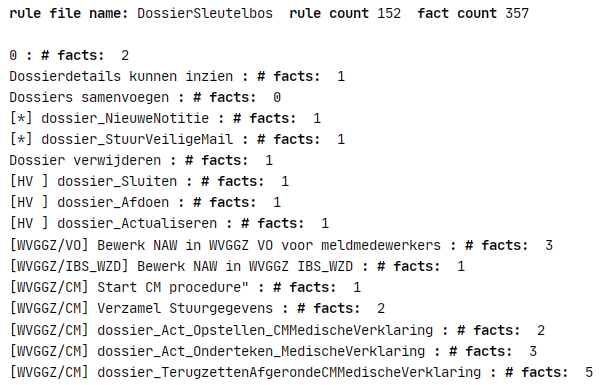
\includegraphics[width=0.66\textwidth]{Sections/images/summaryProjection_P.png}}
    \caption{Summary projection}
    \label{fig:summaryProjection}
\end{figure}

The building of this projection only required adjusting two editors.
The \texttt{Rule} node count and \texttt{FactDeclaration} reference count were added to the \texttt{File} Concept editor using Read-Only Model Access to count the descendants of the \texttt{File} node that are \texttt{Rule} nodes and \texttt{FactDeclaration} references.
The \texttt{Rule} Concept editor was adjusted only to show the \texttt{Rule} nodes title and, again using the model access, the count of the descendants of the \texttt{Rule} that were \texttt{FactDeclaration} references.

Whilst this may look like a report that any language workbench could create, the \texttt{File} node name and the names of the \texttt{Rule} nodes are editable in this projection.

\subsubsection{Filtering}
Whilst investigating how to handle extensive collections of rules, we looked to domains that already handle extensive collections of items.
The domain of data analysis has a long history of handling large volumes.
Among their two most used tools for exploration are sorting and filtering.

The nature of business rules lends them to some projectional options that would not make sense with other programming styles.
Because of the independent nature of the rules, filtering lends itself to the business rules style.
The semantic meaning of the order of business rules means we did not find a good use case for sorting rules.
So, we decided to implement a filtering projection.

Whilst filtering occurs in other places in the coding pipeline, such as deciding on what code completion to present\cite{hou2010towards} and version control visualisation\cite{yoon2013visualization}, we were unable to find any research on applying filtering directly to code files.
Consequently, we think what we present here is an original idea.

\texttt{Rule} nodes that use the same \texttt{FactDeclaration} references or \texttt{FactProperty} references are likely to be related.
Thus, these seemed the obvious items to filter.
We created a projection where if the developer filtered by a \texttt{FactDeclaration} or a \texttt{FactProperty}, the projection would filter out all \texttt{Rule} nodes that did not contain references to the nodes.
Once the \texttt{Rule} nodes were filtered, the projection only shows \texttt{FactDeclaration} nodes and \texttt{FactProperty} nodes that are referenced by those \texttt{Rule} nodes.

In our implementation, shown in figure \ref{fig:filteringProjection} on the following page, we show three places where we use intentions to filter the code.
The first is an intention associated with a \texttt{FactDeclaration} node.
We show the outcome of choosing this filter on the righthand side of figure \ref{fig:filteringProjection}.
The second intention is on a \texttt{FactProperty} node.
As the \texttt{FactProperty} node is a child of a \texttt{FactDeclaration} node, we see both intentions.
The third highlighted intention is on a \texttt{FactProperty} reference.
It also shows an intention associated with a \texttt{FactDeclaration} reference in the \texttt{FactSelector} node that holds the \texttt{FactPropertyReference} as a child.

\begin{sidewaysfigure}
    \centering
    \fbox{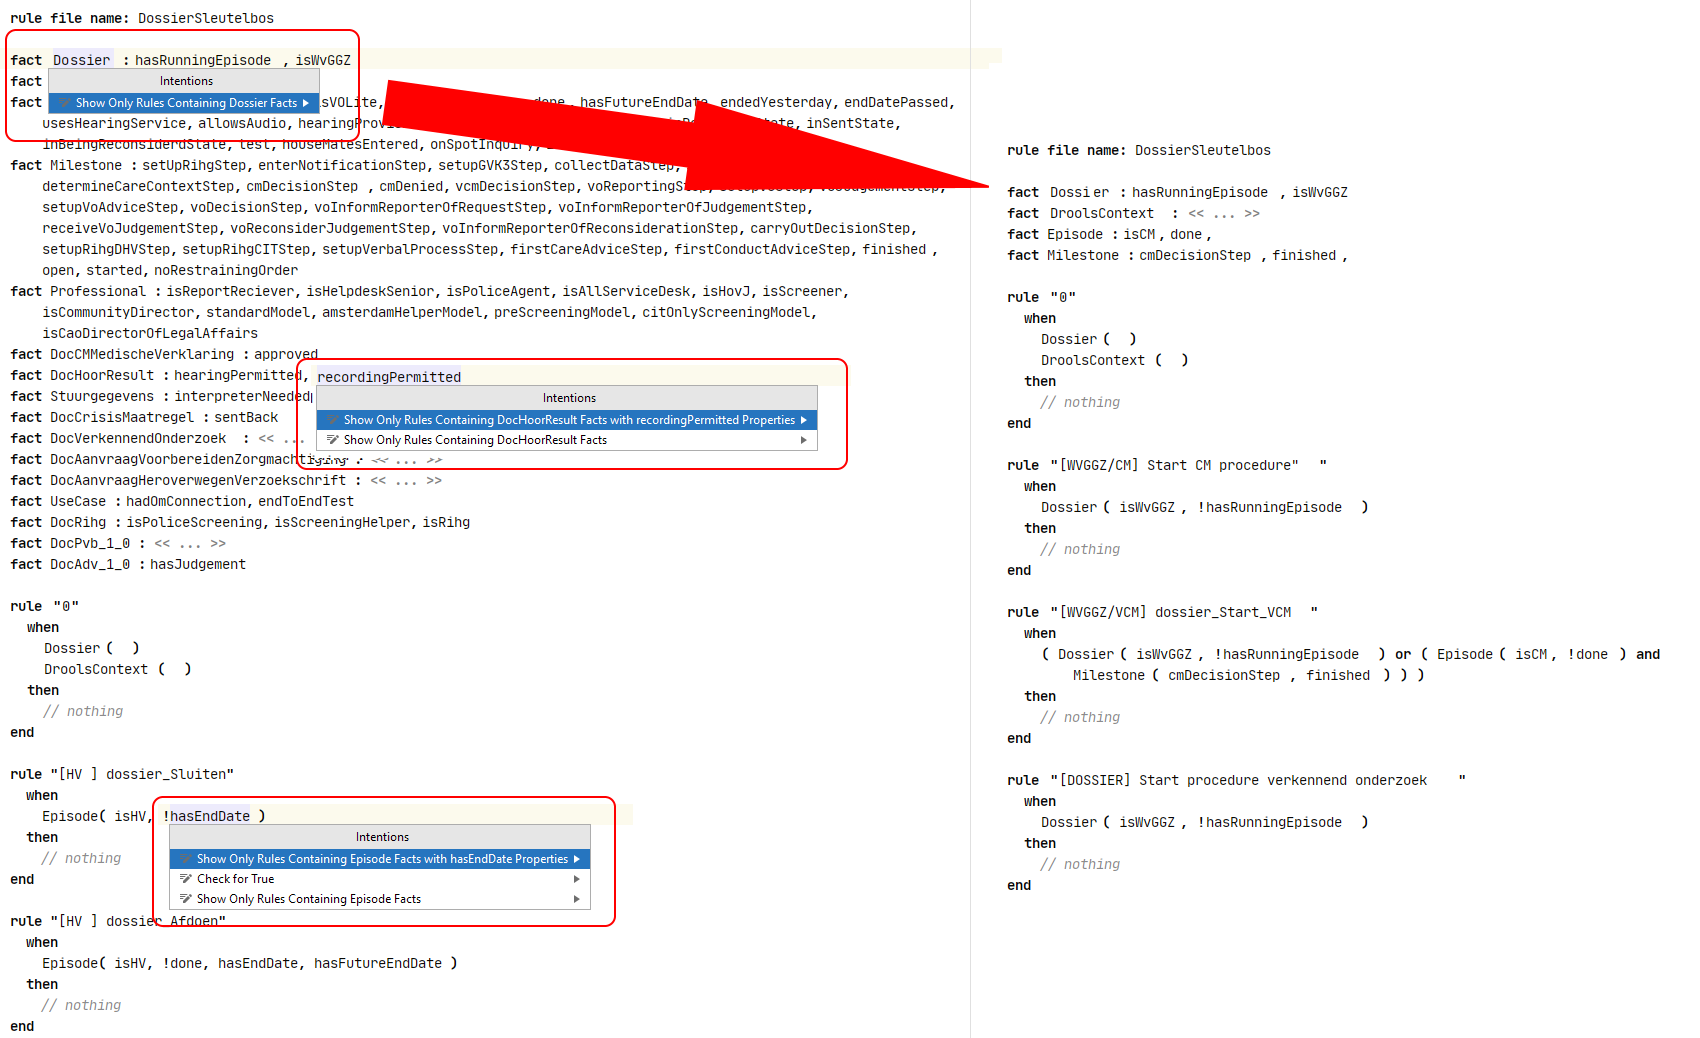
\includegraphics[width=0.99\textwidth]{Sections/images/filteringProjection.png}}
    \caption{Filtering projection}
    \label{fig:filteringProjection}
\end{sidewaysfigure}

One of our guidelines was, as much as possible, to build our projections as separate languages, non-invasively extending RSD.
In our first approach at the filtering, we failed on this count by invasively adding properties to the \texttt{FactDeclaration} and \texttt{FactProperty} Concepts of the RSD to determine whether they were visible.

Our following approach created subclasses of the \texttt{FactDeclaration}, \texttt{FactProperty} and \texttt{File} Concepts.
This approach, however, requires running a macro on the code file to migrate \texttt{FactDeclaration}, \texttt{FactProperty} and \texttt{Files} nodes to \texttt{FilteredFact}, \texttt{FilteredFactProperty}, and \texttt{FilteredFile} nodes.
This migration means that the \texttt{FilteredFile} could now only be used by languages that extend our new filtered language.

Our final approach was to add a \texttt{Filter} Concept, reference the filtered nodes, and have the editors make the visibility calculations based on this singleton node.
Whilst more complex, this removed the need for invasive changes and allowed other languages to combine with the filtering language.

Filtering is a handy projection.
However, it breaks Dijkstra's rule ``the purpose of abstraction is not to be vague but to create a new semantic level in which one can be absolutely precise.''\cite{dijkstra1972humble}.
This projection fails this rule by hiding some of the meaning of the code.
This projection has no way of containing the whole code whilst a filter is applied.
However, we feel that so long as there is a clear indication that a filter is applied, then we see this as a tool in a similar vein to the code collapsing functionality found in most modern-day editors.

\subsubsection{Table}
Thus far, our projections have been textual ones that other non-projectional language workbenches could implement.
Creating a table was our first non-parsable projection.

We choose the table projection based on the observations of Miller\cite{miller1956magical} about the number of items people can retain in their memory.
This observation leads us to conclude that the fewer essential items that are off the screen and, therefore, in the developers' memory, the better.

Figure \ref{fig:tableProjection1} on page \pageref{fig:tableProjection1} shows our rudimentary first table.
This simple table has only the ``name'' property and the ``when'' children of the \texttt{Rule} nodes in the \texttt{File} node.
We implemented this projection using the tables extension in the MPS-Extension plug-in, created by Sascha Lißon.

\begin{sidewaysfigure}
    \centering
    \fbox{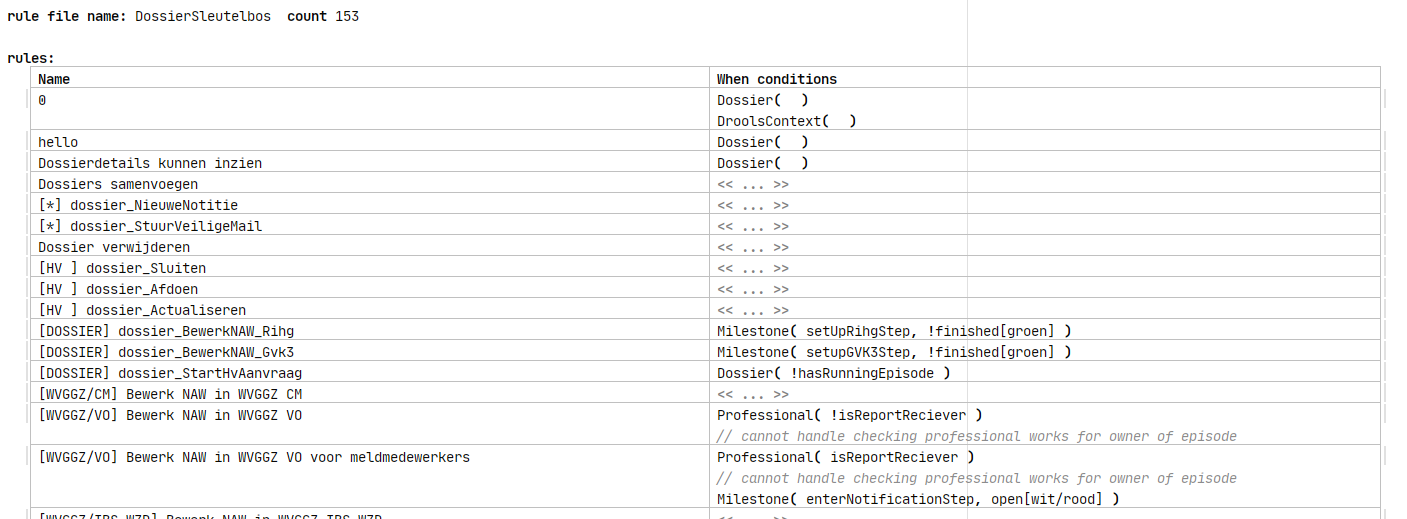
\includegraphics[width=0.99\textwidth]{Sections/images/tableProjection1.png}}
    \caption{Table projection}
    \label{fig:tableProjection1}
\end{sidewaysfigure}

\subsubsection{Crosstab}
Our next tabular projection is a crosstab inspired by a decision table.
Figure \ref{fig:crosstabProjection1}, on page \pageref{fig:crosstabProjection1}, shows our implementation of the crosstab.
Because of the large amount of screen real estate that this projection uses, we only present a truncated view of the table.

The reason behind this projection is that the previous table does not give any visual cues as to how \texttt{Rule} nodes are related.
With a crosstab, one can easily see which rules contain the same facts.

The rows of the crosstab represent the rules, with the name in the left-most column.
The columns represent the facts.

The cells show the facts used in each rule.
A number preceded by a hash symbol indicates if a rile requires a fact.
The number represents the ordinal order of when the facts appear in the conditions.
Thus, the first occurrence of a fact is represented by ``\#1''.
If there are multiple occurrences of a fact within a rule, multiple numbers will appear in the same cell.

In the figure, a close-up shows that all the details of the selected fact are available in the inspector panel.

At the top, we can see an immediate problem with a crosstab
If we have the whole \texttt{File} node represented, then the table will be very sparse.

\begin{sidewaysfigure}
    \centering
    \fbox{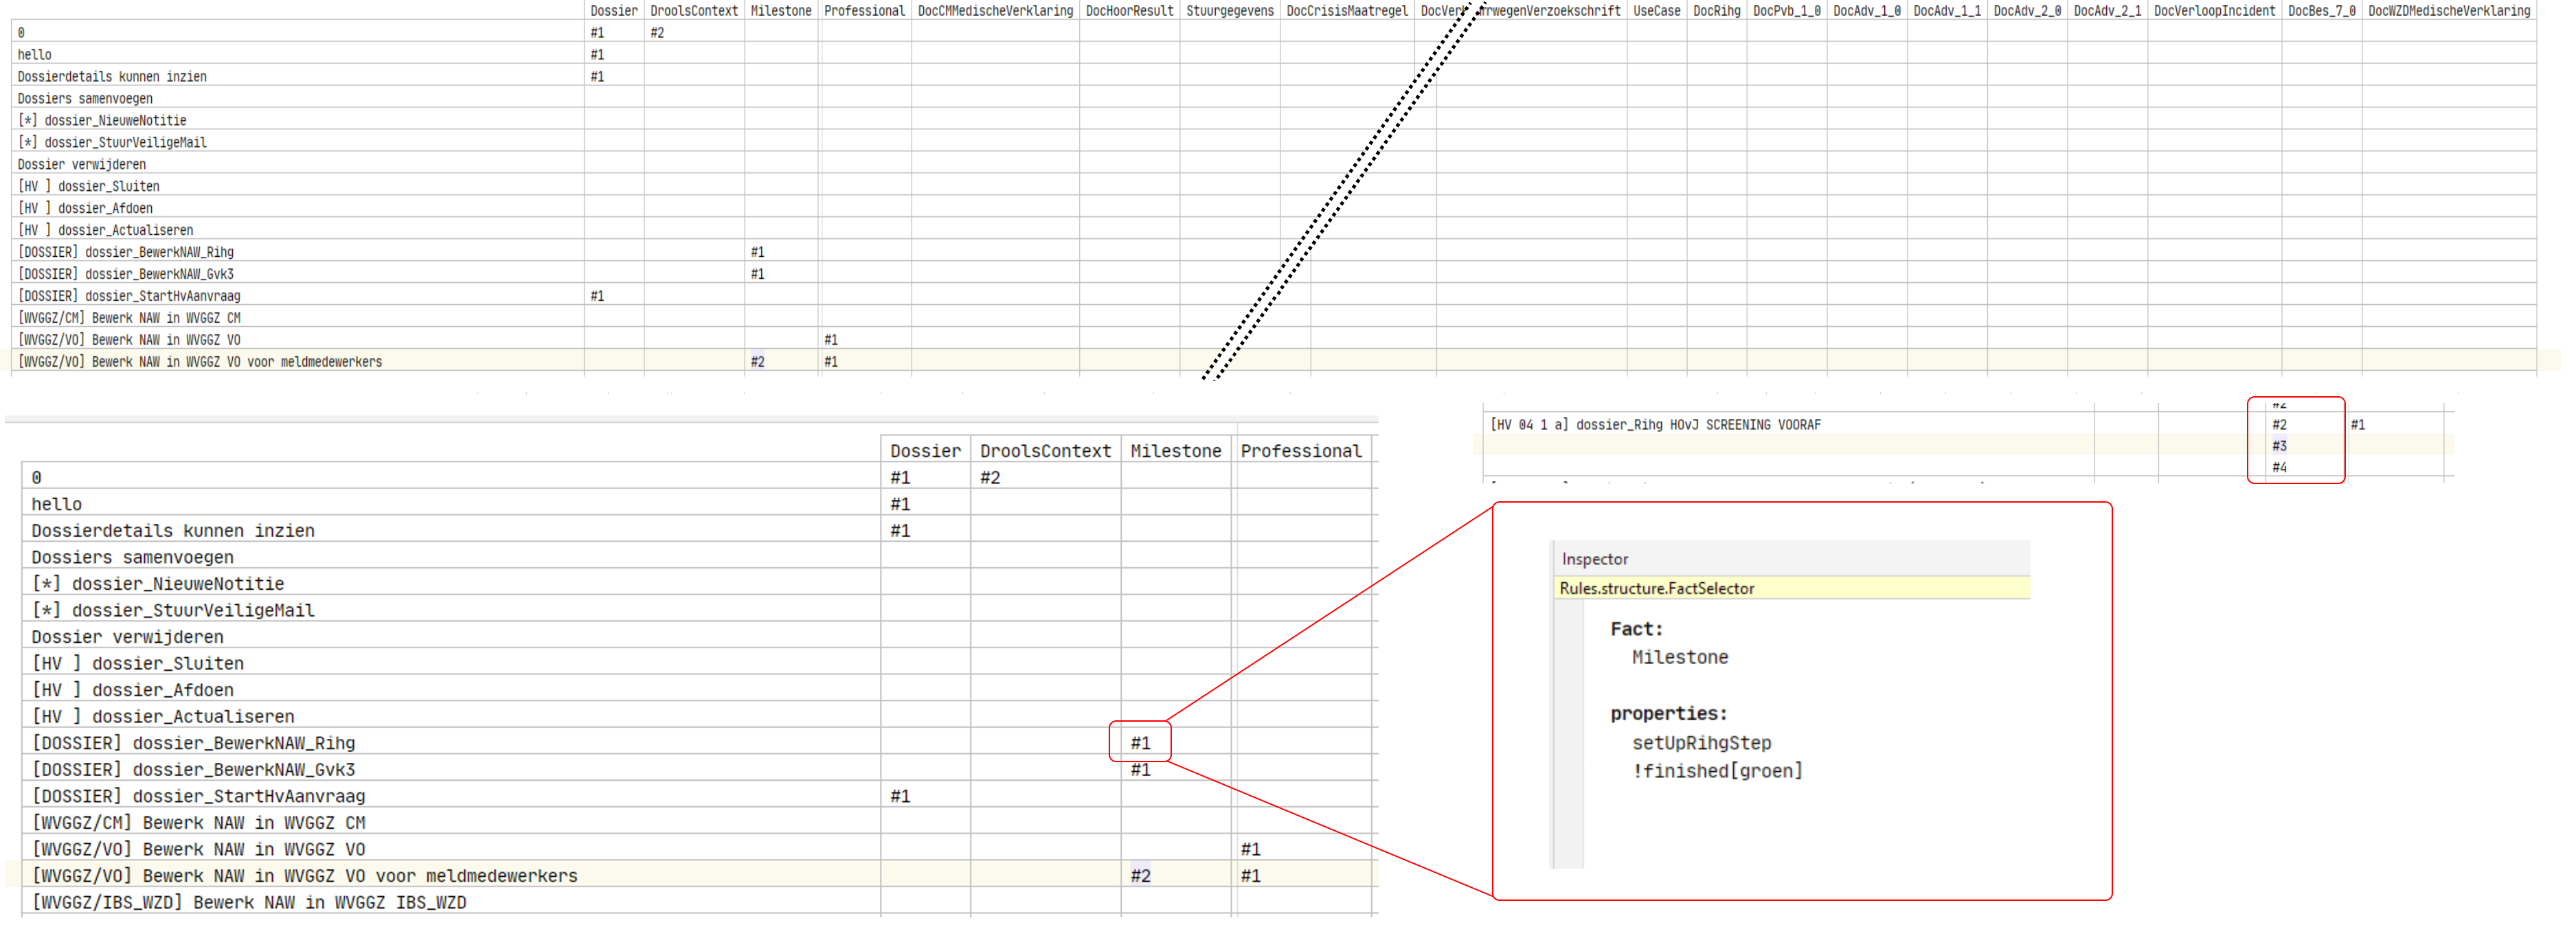
\includegraphics[width=0.99\textwidth]{Sections/images/crosstabProjection1.png}}
    \caption{Crosstab projection}
    \label{fig:crosstabProjection1}
\end{sidewaysfigure}

Everything is editable in this table, including deleting a \texttt{FactDeclarationSmartRef} from a \texttt{Rule} node.
The table plug-in and MPS enabled most of the editing in the projection by default.
An extra editing feature we added to this table was the ability to delete a \texttt{FactDeclaration} node and all the related references from all the \texttt{Rule} nodes in the \texttt{File} node by deleting a fact column.
The code shown in figure \ref{fig:tableFactDeletion}, on page \pageref{fig:tableFactDeletion}, shows how we can walk the trees in each \texttt{Rule} to delete unary conditions and convert the non-deleted side of binary conditions into unary conditions to allow this \texttt{FactDeclaration} reference deletion.

From the ``on delete'' section of the vertical section, we loop through all the \texttt{Rule} nodes to remove the references and rearrange the conditions in the AST.
This projection calls a recursive ``pruneCondition'' method to walk the tree to detach \texttt{FactSelector} nodes containing references to the \texttt{FactDeclaration}.
If it is a unary \texttt{AbstractCondition}, then it detaches the condition, thus removing the contained \texttt{FactSelector}.
Upon removal of both children of a binary \texttt{AbstractCondition}, then the condition is removed.
Upon removing one child from the binary condition, the remaining replaces the parent binary condition.

After removing all the \texttt{FactDeclaration} references, the code removes the \texttt{FactDeclaration}  node that the column represents.
Now that there is an updated AST, the projection will re-display itself. 

\begin{sidewaysfigure}
    \centering
    \fbox{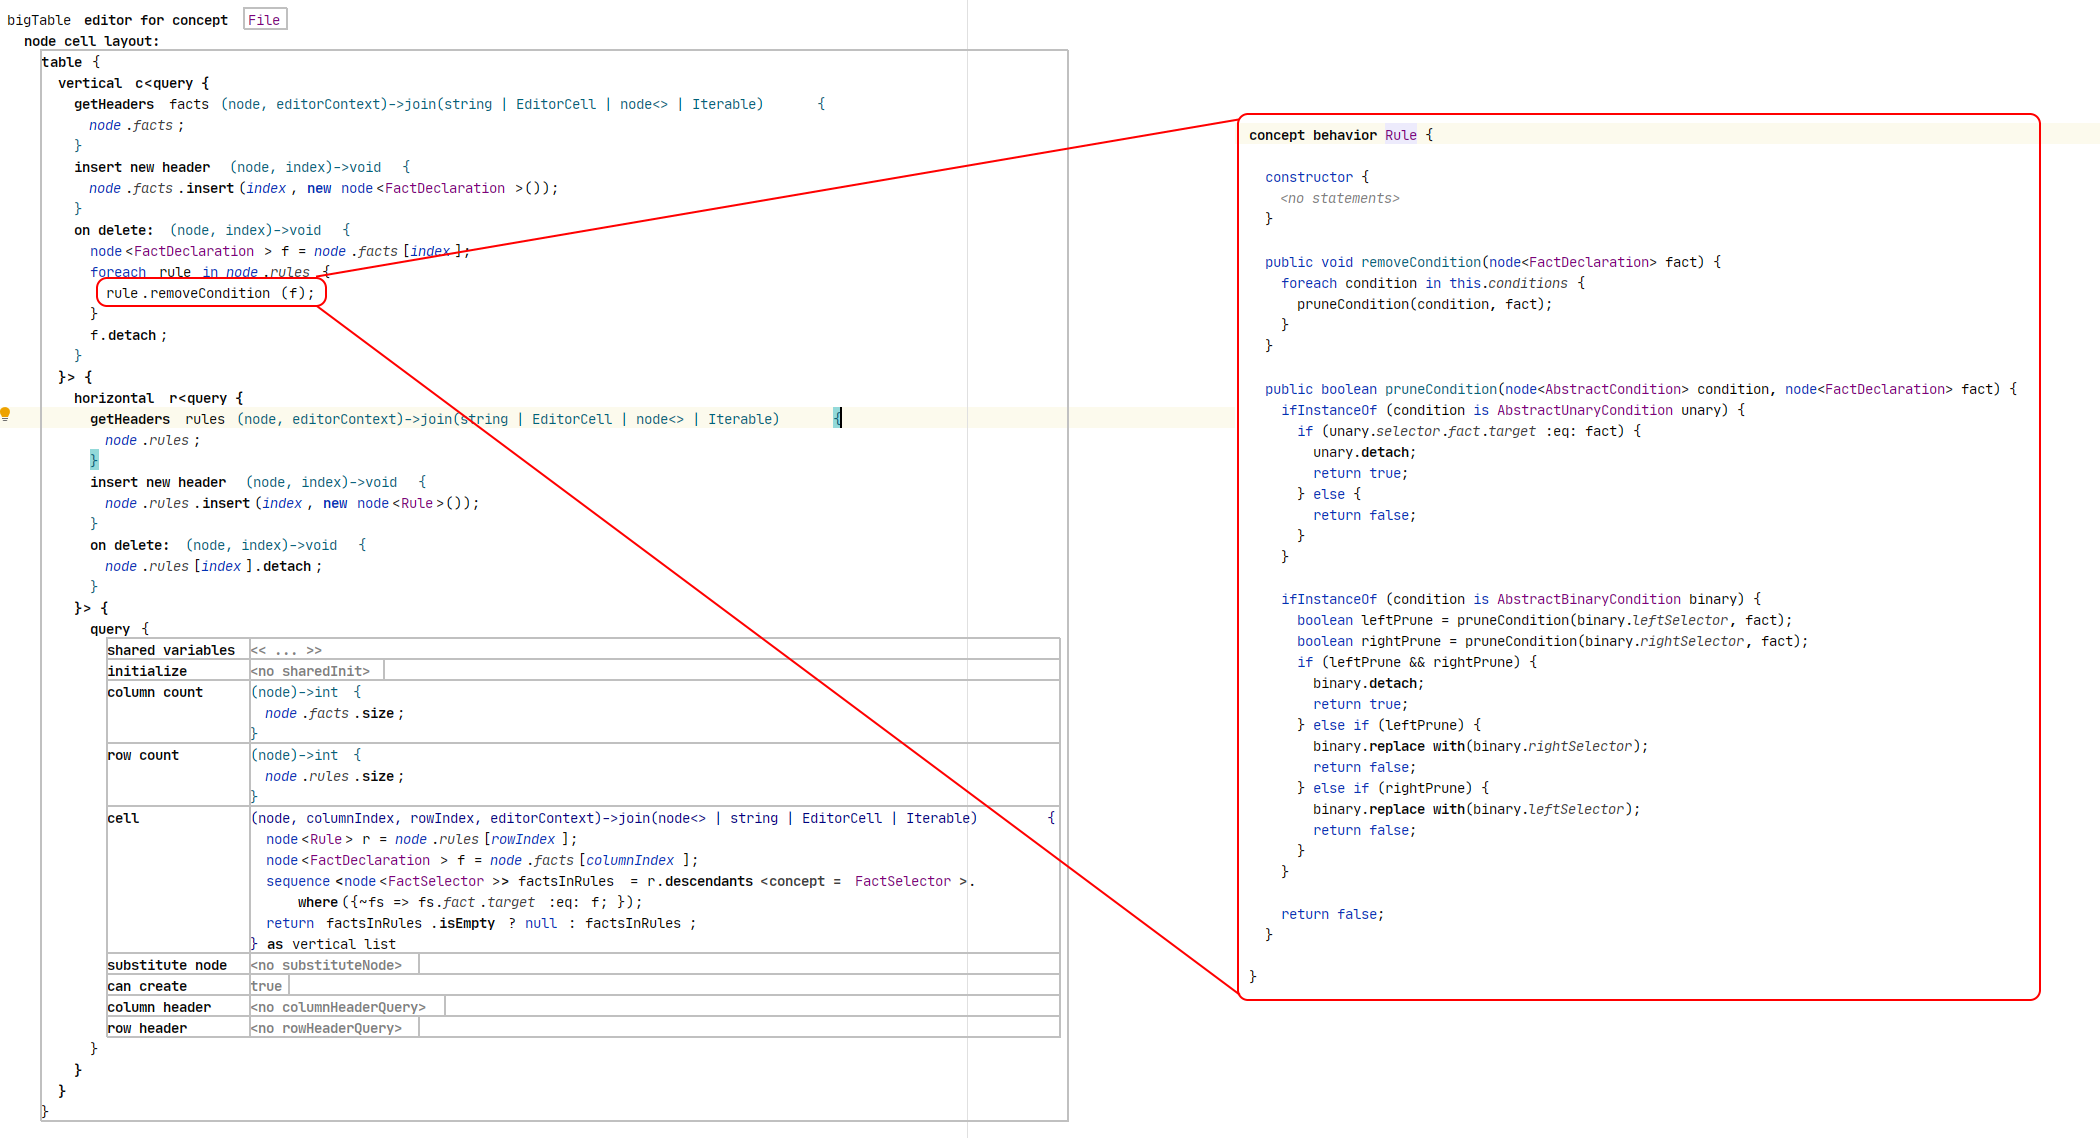
\includegraphics[width=0.99\textwidth]{Sections/images/tableDeleteCode.png}}
    \caption{Table Fact deletion code}
    \label{fig:tableFactDeletion}
\end{sidewaysfigure}

Here we end our experiments in the RSD language.

\newpage

\subsection{Drools-Lite}

Our subsequent experiments were with projections with the Drools-Lite language.
As described in section \ref{section:DroolsLite}, Drools-Lite is an implementation that is much closer to the complete Drools language.
This realism will allow us to create projections that we can present to experienced Drools developers for evaluation.

Of the learnings from the RSD language, one we felt needed fixing to improve understanding was the sparseness of the tables.
By implementing the principle of maximising cohesion, we discovered we could reduce the sparseness issue.
Therefore, as a precursor to our projections, we extended Drools-Lite with a new language that contained one structural item - the \texttt{RuleCollection} Concept.
A \texttt{RuleCollection} node is a child of the \texttt{File} Concept and holds a collection of \texttt{Rule} nodes.
This idea is that related \texttt{Rule} nodes can be placed in the \texttt{RuleCollection}  node to make it easier to examine them together.
This language naturally also added an editor for the \texttt{RuleCollection} Concept.
Additionally, we added intentions to move \texttt{Rule} nodes in and out of groups.

\subsubsection{Decision Table}

As the Drools language is analogous to a series of if-then statements, then perhaps its best visual equivalent is the decision table.
Decision tables are a ``powerful aid in programming, documentation, and in effective man-to-man and man-to-machine communications''\cite{pooch1974translation}.

We designed our table, shown in figure \ref{fig:decisionTableProjection}, to include some of the lessons learned from the RSD crosstab shown in figure \ref{fig:crosstabProjection1}.
The RSD language taught us that wasting visual real estate exacerbates sparseness issues in tables.
In the crosstab table, horizontal scrolling is necessary, in part due to the column widths.
The columns were wide because the name of the \texttt{FactDeclaration} node was displayed horizontally.

\begin{figure}[h]
    \centering
    \fbox{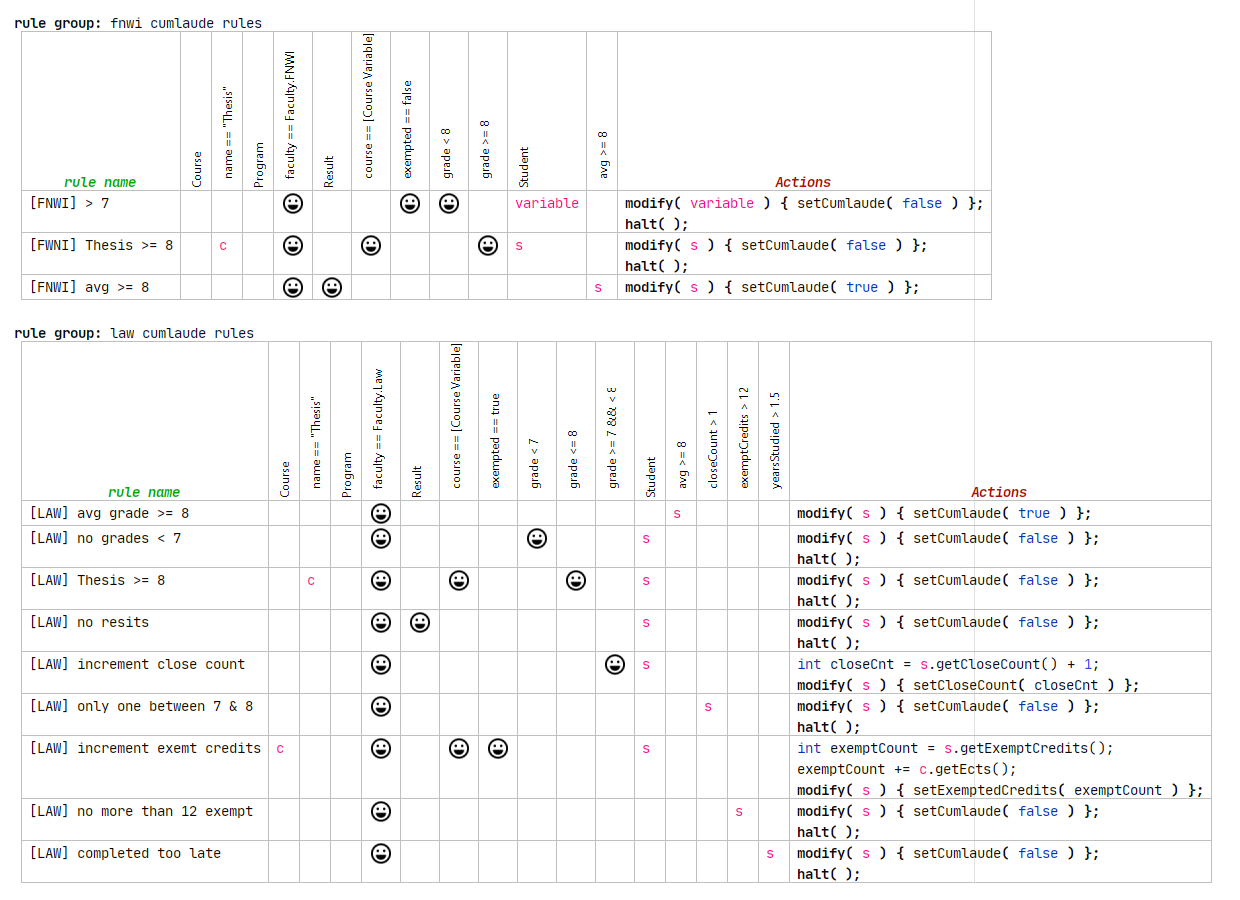
\includegraphics[width=0.99\textwidth]{Sections/images/decisionTableProjection.png}}
    \caption{Decision table projection}
    \label{fig:decisionTableProjection}
\end{figure}

The Drools-Lite language allows for much longer selection criteria on \texttt{FactProperty} references, which would lead to much wider columns.
Our solution was to develop a vertically orientated header cell and use indentation to indicate if the cell is referring to just the \texttt{FactDeclaration} node or a \texttt{FactDeclaration} and \texttt{FactProperty} node combination.

Because this projection presents both the left and right-hand side of the rules, we had to handle the Concept that spans both - the \texttt{RuleVariable} Concept.
We had to find a way to represent a \texttt{RuleVariable} node that can be bound and used on the LHS and used on the RHS.
We achieved this by referencing a \texttt{RuleVariable} node's name in the cell representing the \texttt{FactDeclaration} reference or \texttt{FactProperty} reference to which it is bound.
With \texttt{RuleVariable} nodes now being represented in the cells, we could no longer represent the cell being selected with an ``X'', as this could be confused with a \texttt{RuleVariable} node's name.
Projectional editing does not require communication of meaning through parsable ASCII text.
Thus, we decided to represent \texttt{FactDeclaration} nodes selection with an image.
For arbitrary reasons, we chose a smiley face as that indicator.

The \texttt{Rule} node's names and actions are editable through the default functionality of the MPS extension.
We use intentions to add the selection of a \texttt{FactDeclaration} node or \texttt{FactProperty} reference to a \texttt{Rule} node.
We also use intentions for binding \texttt{RuleVariables}.

The major drawback of this design is that editing a \texttt{Rule} node with yet non-existent selection criteria became very clunky.
If the \texttt{Rule} node we wished to edit already existed in the table, we had to use an intention to extract it from the group, change the criteria and place it back in.
At this point, the table would automatically adjust the column headings.

Experts examined this design in the questionnaire.

\subsubsection{SpreadSheet}

The domain-specific language for the finance world is the spreadsheet.
One study estimated that 90\% of computers had a spreadsheet on them\cite{bradley2009using}.
Dan Bricklin's VisiCalc drove personal computers into the office.
VisiCalc was succeeded by Lotus 1-2-3, which Microsoft Excel then succeeded as the dominant spreadsheet program in the workplace.

This level of familiarity with a paradigm led us to design a projection that had the look and feel of an Excel spreadsheet.
We show this design in figure \ref{fig:SpreadsheetProjection}.
To this end, we created a design where the selection criteria could be directly edited in the cell, as highlighted in the figure.

Each row is a \texttt{Rule} node in this design, and each column is for a \texttt{RuleVariable} node or a \texttt{FactProperty} reference.
If a property is selected, then the selection criterion is in the appropriate cell.
A grey/beige colour indicates unselected cells.
The RHS of the \texttt{Rule} node appears in the Action column.
Adding as yet unused \texttt{FactDeclaration} references or \texttt{FactProperty} references, or removing existing ones, can be achieved with intentions, as shown in figure \ref{fig:SpreadsheetIntentions}, on page \pageref{fig:SpreadsheetIntentions}.

\begin{figure}[h]
    \centering
    \fbox{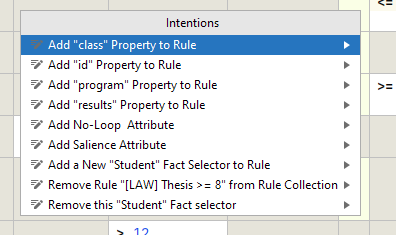
\includegraphics[width=0.55\textwidth]{Sections/images/spreadsheetIntentions.png}}
    \caption{Intention}
    \label{fig:SpreadsheetIntentions}
\end{figure}

This design also allowed us to have more than one selector for the same \texttt{FactProperty} reference, essential for our host organisation's code.
We demonstrate this in figure \ref{fig:TwoProperties}.

\begin{figure}[h]
    \centering
    \fbox{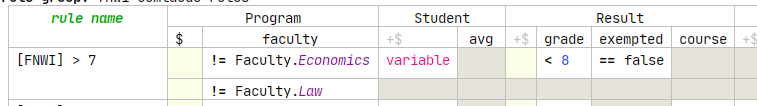
\includegraphics[width=0.90\textwidth]{Sections/images/spreadsheetTwoProperties.png}}
    \caption{Two of same property}
    \label{fig:TwoProperties}
\end{figure}

Experts examined this design in the questionnaire. 
Here we end our experiments in the Drools-Lite language.

\begin{sidewaysfigure}[htbp]
    \centering
    \fbox{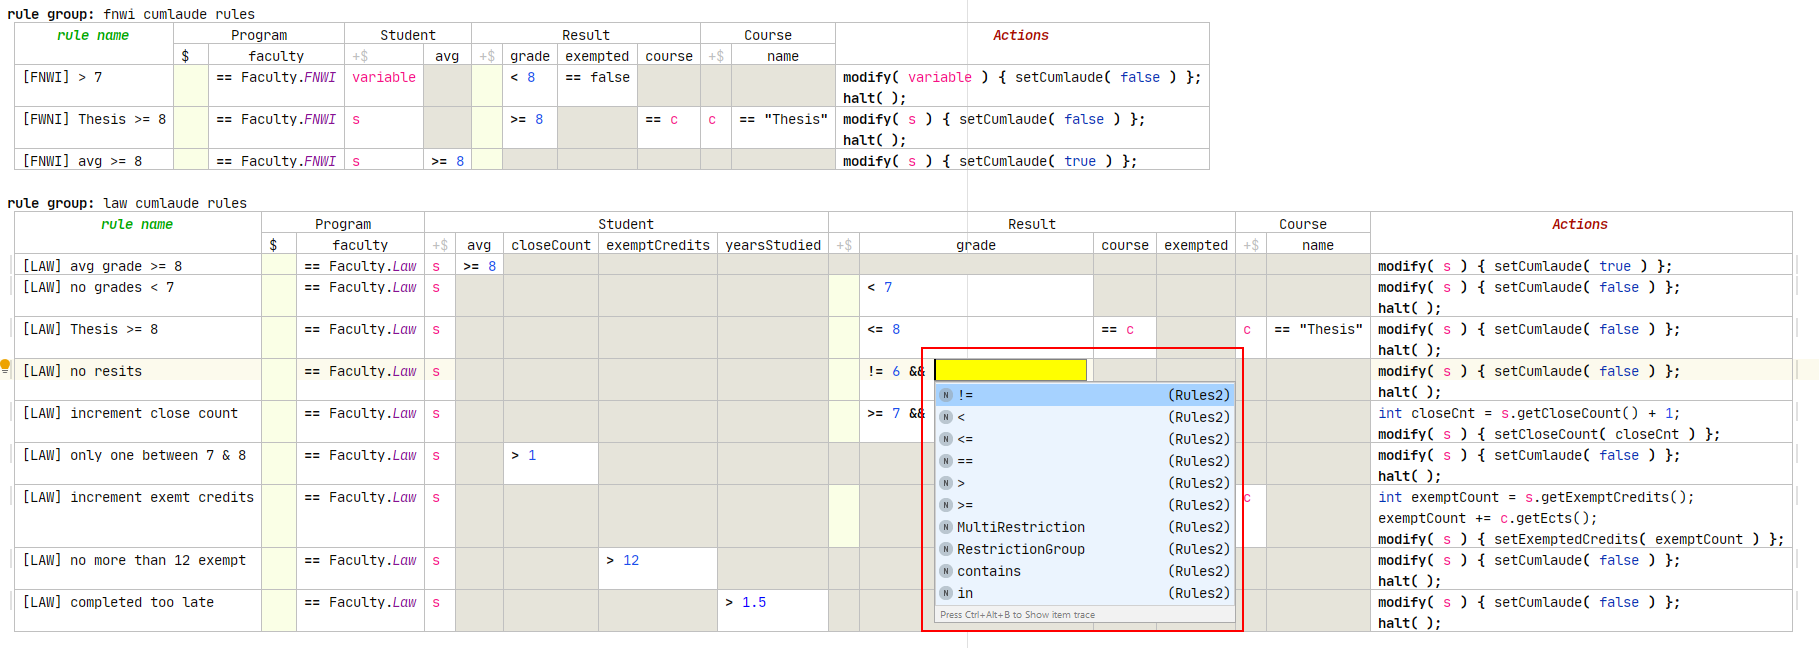
\includegraphics[width=0.99\textwidth]{Sections/images/SpreadsheetProjection.png}}
    \caption{Spreadsheet projection}
    \label{fig:SpreadsheetProjection}
\end{sidewaysfigure}

\newpage

\subsection{Wireframe}

After brainstorming several ideas to present as wireframes to experts as possible projectional aids to understanding, we chose two.
We discuss them briefly in this section.

\subsubsection{Truth Table}
We decided to produce a truth-table wireframe example as we had had personal experience building truth tables to confirm the validity of Drools rules in our work.

The truth table seemed apt for the LHS of the Drools rule as, in essence, it is a boolean function.
Wittgenstein popularised the truth table in the Tractatus Logico-Philosophicus\cite{wittgenstein2013tractatus}.
They are so widely used in mathematics and computer science that we do not need to explain their use further.
Because of the combinatorial explosive nature of truth tables, with 2\textsuperscript{n} possible combinations, we would limit the display to a max of 6 \texttt{FactSelector} nodes and only show the paths that lead to the RHS execution.

Figure \ref{fig:TruthTableProjection} shows how we designed this to look.
The user experience would be that the \texttt{Rule} node is selected, and the developer presses the up and down arrow keys to step through the different true (highlighted in green) and false (highlighted in red) \texttt{FactSelector} nodes that result in the \texttt{Rule} nodes selection.

\begin{figure}[h]
    \centering
    \fbox{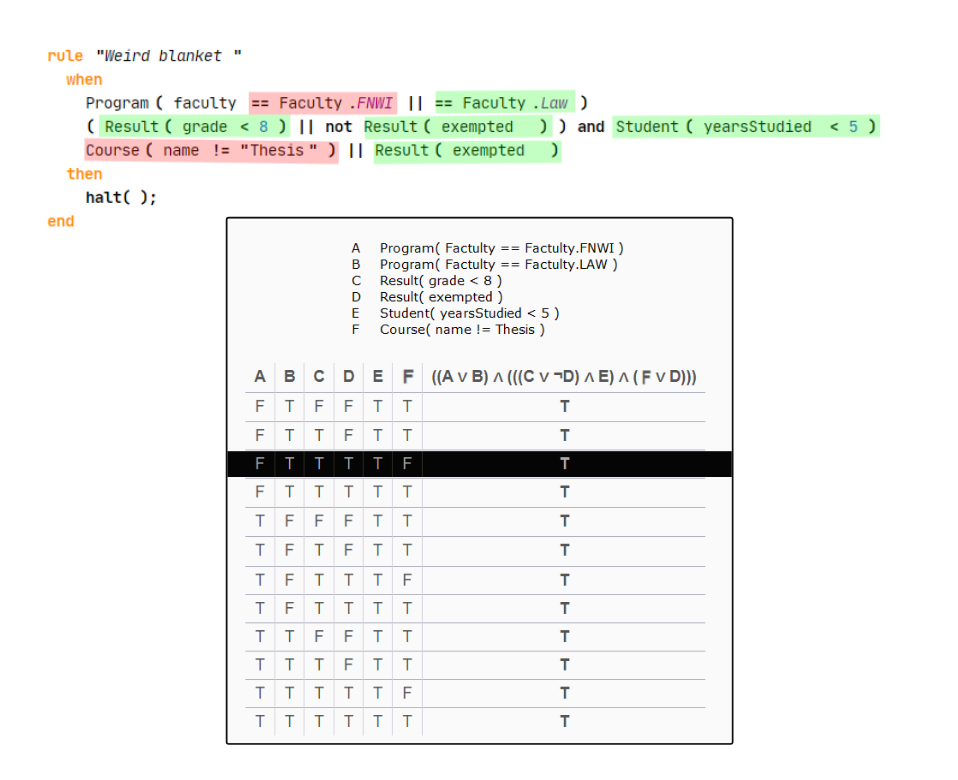
\includegraphics[width=0.80\textwidth]{Sections/images/truthtable.png}}
    \caption{Truth table projection}
    \label{fig:TruthTableProjection}
\end{figure}

We presented this design to our experts to be validated.

\subsubsection{Circuit Diagram}
In our final projection design, we wanted to present a part of projectional editing that we had heretofore only made minimal use of.
That is the use of manipulatable graphics that can change the AST.

We chose a logic circuit. 
The logic circuit represents a boolean operation as NOT, OR, XOR and AND Gates, with their inputs and outputs being inputs to other gates.
In our design, shown in figure \ref{fig:CircuitDiagramProjection}, the input wires to the gates are the \texttt{FactDeclaration} nodes or \texttt{FactProperty} nodes referenced in the LHS.

\begin{figure}[h]
    \centering
    \fbox{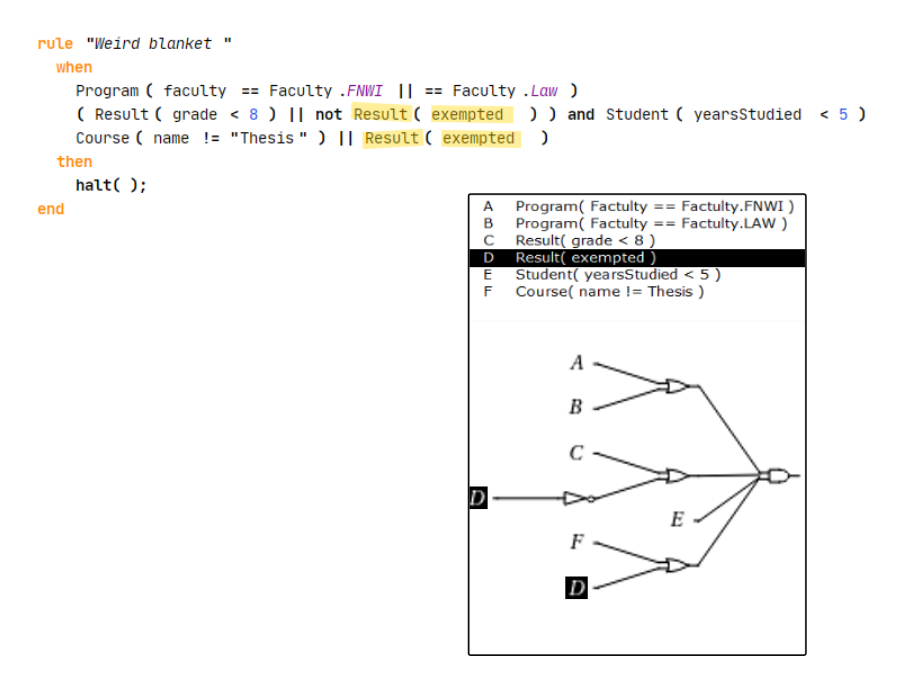
\includegraphics[width=0.80\textwidth]{Sections/images/CircuitDiagram.png}}
    \caption{Circuit diagram projection}
    \label{fig:CircuitDiagramProjection}
\end{figure}

The user experience is that once the \texttt{Rule} node is selected, the developer, by pressing the up and down arrow keys, can step through the different \texttt{FactSelector} nodes (highlighted in yellow) and shown in the circuit diagram, thus showing how the \texttt{FactDeclaration} nodes relate to each other.

We present this design in the questionnaire for validation.



\section{Discussion}
\label{section:dsr_discussion}

We now examine threats to the construct, the internal and external validity of our DSR, its reliability, and areas of improvement.


\subsection{Threats To Validity} 

\subsubsection{Conclusion Validity}
We felt that the projections we built improved our overview of large rule sets.
However, as we spent a lot of time with the rules as the projections are being built, we could have been influenced by the previous knowledge of the rules.
Thus, we needed to validate our conclusions with others, which chapter \ref{chapter:Survey} attempts to do.

\subsubsection{Construct Validity}
We were trying to observe whether projectional techniques could help with understanding Drools rules. 
As some of the outcomes could have also been achieved with other, non-projectional, language workbenches, these did not contribute to proving a link between better understanding and projectional editing.
As the tabular projections would not be achievable in parser based languages, then these could show the direct relationship between projections and understanding.

\subsubsection{Internal Validity}
If there was a better understanding, was this the result of the tabular projectional editing?
There are many advantages that come from the implementation in MPS, these include the context aware code completion menus.
Some of these side effects, rather than the core concept, could have impacted our understanding.

\subsubsection{External Validity}
Our Drools-Lite language is not a full implementation of the Drools language.
To take in the whole language would have taken more time.
Whether the examples we built would generalise to all the functionality of Drools is not known. 

\subsubsection{Reliability}
Reliability is how the data and the analysis is dependant on specific researchers.
With DSR studies, that build a working opensource prototype, then the reliability of the data is known.
The code can just be downloaded and run by any interested party.  

The reliability of our analysis, that the projections improved our understanding, is be open to effects of a range of cognitive biases.
To take out the effect of our biases this we surveyed others, as described in chapter \ref{chapter:Survey}.

\subsubsection{Repeatability Vs Reproducibility}
Implementing ideas in code can take

\subsubsection{Method Improvement}

\section{Summary}
In this chapter, we presented a description of the details of the DSR that we conducted.
We pursued two languages.
In our pilot study, we implemented the Really Simple Drools language and a few projections on top of this.
Once we had established the usefulness of this approach, we created the language Drools-Lite which was a language that would be recognisable to experienced Drools developers.

Of the projections we created, the most capable were the Spreadsheet-like and Decision table-like projections.
These both succeeded in massively reducing the screen real estate required.
Other advantages included being able to group related rules and being able to visually scan which rules used the same facts and properties.

We could not show rules with complex nested conditions in the tabular projections — however, the ability to mix notations mitigated this.
We could show rules too complicated for the tabular projections with textual projections in the same file.